
\subsection{UART Implementation}
The UART is interrupt driven. The interrupt fires when you call uart\_write(uint8\_t*, int) to signify that the buffer is non empty by setting a non empty flag. There are two pointers that point at the beginning and end of the buffer, head and tail. Each character/byte is sent individually until the head == the tail and the empty flag is restored.

\lstset{language=c}
\lstset{commentstyle=\textit}
\begin{lstlisting}[frame=trbl]{}
int uart_write(uint8_t* const str, int len){
    int overflow = 0;
    int i;

    uint8_t sreg;
    sreg = SREG;

    Disable_Interrupt();
    overflow = 0;
    for(i = 0; i < len; ++i){  
        if(non_empty && head == tail) overflow = -1;

        uart_TX_buf[tail] = str[i];

        ++tail;
        tail &= UART_TX_BUF_MASK;
    }
    
    if(overflow) head = tail;     

    if(len > 0) {

        TXIntEnable();
        non_empty = 1;
    }

    SREG = sreg;
    return overflow; 
}

/**
 * Interrupt service routine for the UART transmission.
 */
ISR(USART1_UDRE_vect) {
    UDR1 = uart_TX_buf[head];
    ++head;
    head &= UART_TX_BUF_MASK;
    // Last byte was written?
    if (head == tail){
        non_empty = 0;
        TXIntDisable();
    }
}
\end{lstlisting}

The simplist way for UART to be used, is to create a character buffer and insert the desired String using sprinf. This made is very simple to monitor length and insert decimals. 

\lstset{language=c}
\lstset{commentstyle=\textit}
\begin{lstlisting}[frame=trbl]{}
int len = sprintf((char *)toPrint, "X %d, Y %d\r\n", packet->x, packet->y);
uart_write((uint8_t*)toPrint, len);
\end{lstlisting}

\subsection{DC Motor Implementation}

\subsubsection{Initialization}
The D/C motor uses Pulse Width Modulation(PWM) to determine the speed at which it turns. This PWM is sent through the enable pin of the H-bridge. There is also a direction pin which must be set to either high or low.

This pin is set as output to be able to turn the motor on and off.
\lstset{language=c}
\lstset{commentstyle=\textit}
\begin{lstlisting}[frame=trbl]{}
 DDRD |=  (1< < PORTD7);
\end{lstlisting}

This pin is the direction pin, also set to output. 

\lstset{language=c}
\lstset{commentstyle=\textit}
\begin{lstlisting}[frame=trbl]{}
 DDRC |= (1< < PORTC1);
\end{lstlisting}

Finally, this pin is the pin that outputs the PWM, also set for output. 

\lstset{language=c}
\lstset{commentstyle=\textit}
\begin{lstlisting}[frame=trbl]{}
DDRB |= (1< < PORTD7);
/** setup timer/counter 0  for fast PWM   **/ 
TCCR0A = (1 < < WGM00) | (1 < < WGM01) | (0 < < COM0A0) | (1 < < COM0A1);
TCCR0B = (0 < < WGM02) | (0 < < CS02) | (0 < < CS01) | (1 < < CS00);
\end{lstlisting}

The COM0A1..0 pins control the output of OCA0. In the motor driver, the compare output mode is set to clear OC0A when the counter matches the value in the output compare register, OCR0A, and to pull high when the counter reaches the TOP value. By setting and clearing OCA0, the pulse width that drives the motor is generated. According to the AT90USB1287 datasheet, different modes of operation will have different effect on the behavior of OC0A. The operation mode we are using is Fast PWM mode. It can be set by setting WGM02..0 to 011. The last thing that the motor initialization function does to set the clock prescaler. CS02..0 determines the prescale factor. For us, we set CS02..0 to 001 which disables the prescaling.

\begin{figure}[h]
  \begin{center}
    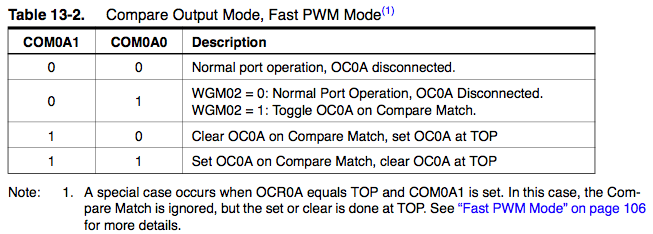
\includegraphics[width=125mm]{imageSources/pwmTable1.png}
  \end{center}
  \caption{Fast PWM Mode} 
  \label{pwmTable1}
\end{figure}

The above table outlines the 8 different types of  Waveform generation that are available. As can be seen by how we set the code, we chose to use mode7. This describes that the system uses fast PWM and that the top value is defined by OCRA.  As can be seen in the following section, we change the value of OCR0A to  change the speed of the motor.

\begin{figure}[h]
  \begin{center}
    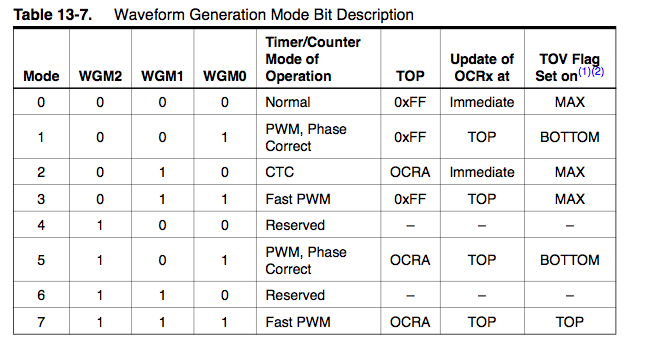
\includegraphics[width=125mm]{imageSources/waveformGenerationTable.png}
  \end{center}
  \caption{Waveform Generation Mode Bit Description} 
  \label{waveformGenerationTable}
\end{figure}
